%!TEX root = ../document.tex
\chapter{Vorbereitung}

\section{Installationsanleitung Live USB mit Persistenz}

Es wurde ein Live USB erstellt, von welchem wir Kali Linux starten. Dies bedeutet, dass wir ein Kali Linux Image auf einen USB-Stick übertragen und von diesem dann anschließend auch das Kali Linux Betriebssystem booten können. 
Durch die zusätzliche Persistenz können Änderungen und Daten, die auf dem USB-Stick gespeichert werden, gespeichert werden und stehen somit auch nach einem Neustart des Kali Linux Systems zur Verfügung.

\subsection{Ablauf des Vorgangs mit Win10}

Es sollte mindestens ein 8GB USB-Stick verwendet werden.
!!WARNUNG ES GEHEN ALLE DATEN AUF DIESEM USB-STICK VERLOREN!!

Im diesem Abschnitt wurde folgendes verwendet

\begin{itemize}
	\item \bashCommand{SanDisk Ultra USB 3.0 16GB} USB-Stick der bootbar gemacht wird
	\item \bashCommand{Kali linux 2016.2 64bit} ISO-File Kali Linux
	\item \bashCommand{MiniTool Partition Wizard 9.1} Formatieren und Anpassen der Partitionen
	\item \bashCommand{Universal USB Installer 1.9.6.8} Übertragen des Images auf den USB-Stick
\end{itemize}

Zuerst muss die aktuellste Version von Kali Linux heruntergeladen werden. Diese kann man auf www.kali.org/downloads/ finden.
Sollten sich noch Daten auf dem USB-Stick befinden bitte diese jetzt an einem anderem Ort abgespeichert und dann vom USB-Stick entfernt werden. 
Um nun das Kali Image auf den USB-Stick zu übertragen wird der Universal USB Installer geöffnet.

Nun sollten wie in Abbildung \ref{fig:start usb installer} in Step 1 Kali Linux ausgewählt werden. In Step 2 muss nun der "'Browse"' Button betätigt und der Pfad der Kali ISO-Datei ausgewählt werden. Anschließend wird in Step 3 der gewünschte USB-Stick ausgewählt werden. Dabei sollte auch das Kästchen daneben ausgewählt werden, um den USB-Stick auf Fat32 zu formatieren. (Achtung! Hier bitte sorgfältig arbeiten, sonst könnte die falsche Partition gelöscht werden.)
	\begin{figure}[H]
		\centering
		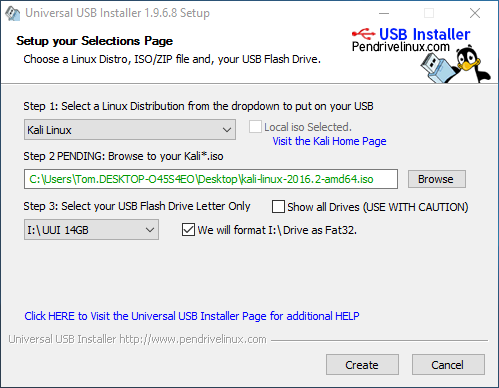
\includegraphics[width=0.7\textwidth]{images/prep/start_usb_installer.png}
		\caption{Einstellungen beim Universal USB Installer}
		\label{fig:start usb installer}
	\end{figure}


Nach erfolgreichem Abschluss öffnen wir nun das Programm MiniTool Partition Wizard. Hier muss nun wie in Abbildung \ref{fig:rightclick resize} per Rechtsklick auf den Speicherbereich des USB-Sticks "'Move/Resize"' ausgewählt werden.
	\begin{figure}[H]
		\centering
		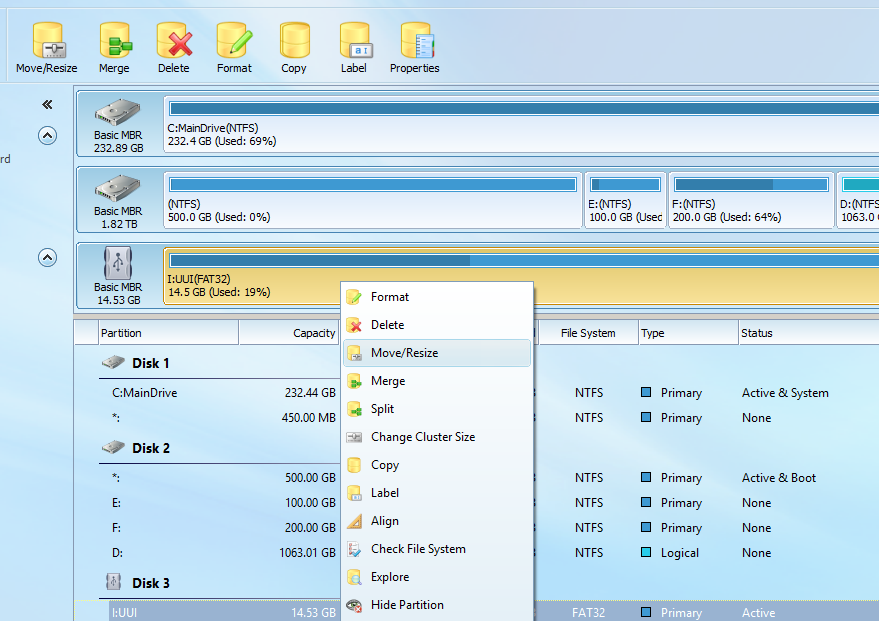
\includegraphics[width=0.8\textwidth]{images/prep/click_resize_part.png}
		\caption{Rechtsklick auf den Speicherbereich}
		\label{fig:rightclick resize}
	\end{figure}
Im nächsten Fenster soll der Speicherbereich der Partition verkleinert werden.
	\begin{figure}[H]
		\centering
		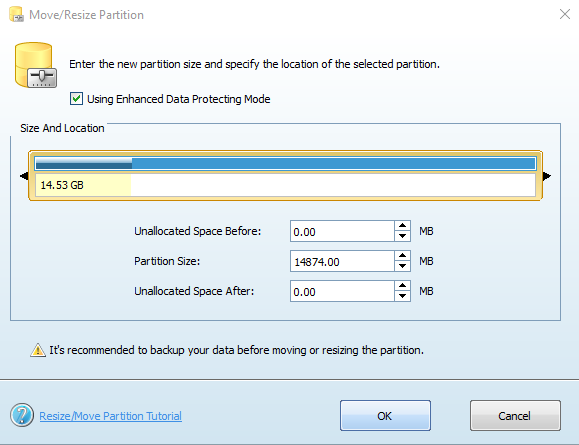
\includegraphics[width=0.75\textwidth]{images/prep/resize_window.png}
		\caption{Verkleinern der Partition}
		\label{fig:start resize partition}
	\end{figure} 

	\begin{figure}[H]
		\centering
		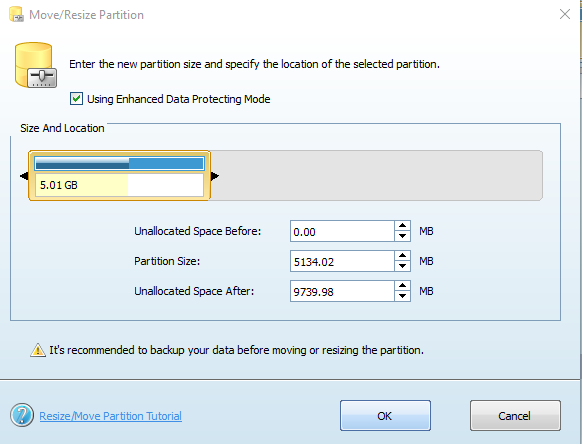
\includegraphics[width=0.75\textwidth]{images/prep/resized_part.png}
		\caption{Verkleinern der Partition}
		\label{fig:finish resize partition }
	\end{figure} 
Für unser Beispiel wurden 5GB ausgewählt, obwohl noch kleinere Werte auch möglich wären.
Nachdem dieser Vorgang ausgeführt wurde, ist nun ein grauer, nicht belegter Bereich sichtbar.
Nach Rechtsklick auf diesen Bereich und anschließendem Klick auf "'Create"' öffnet sich ein neues Fenster.
	\begin{figure}[H]
		\centering
		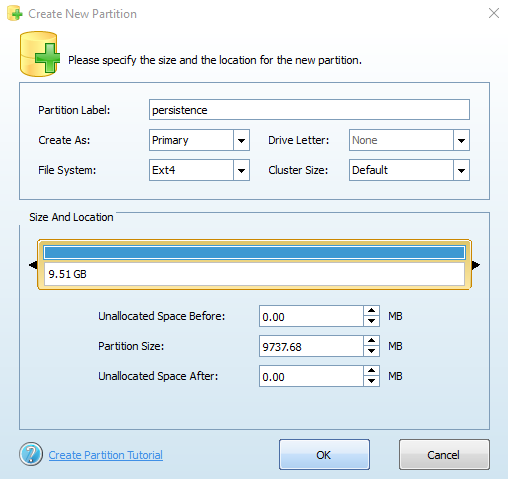
\includegraphics[width=0.9\textwidth]{images/prep/create_part.png}
		\caption{Erstellen der zweiten Partition}
		\label{fig:createPartition}
	\end{figure}

Wie in Abbildung\ref{fig:createPartition} müssen nun die folgenden Optionen ausgewählt werden. 

\begin{itemize}
	\item Partition Label: persistence
	\item Create as: Primary
	\item File System: Ext4
\end{itemize}

Um alles auszuführen, muss im linken oberen Teil des Fensters auf "'Apply"' gedrückt werden.
Nachdem dieser Vorgang abgeschlossen wurde, beenden sie den Partition Wizard.

Nun muss der PC neu gestartet werden und vom neu erstellten USB-Stick gebootet werden.
Beim Bootvorgang sehen wir nun folgendes Fenster.

	\begin{figure}[H]
		\centering
		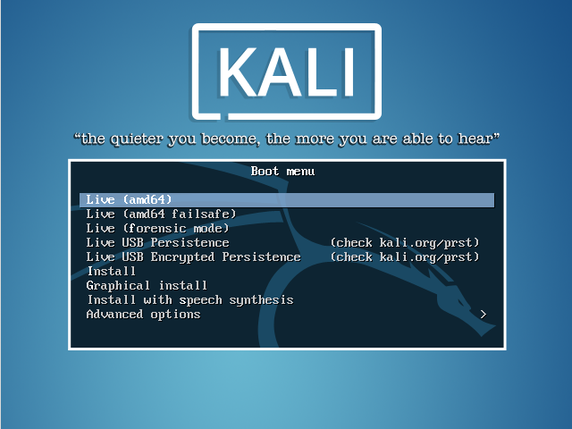
\includegraphics[width=0.9\textwidth]{images/prep/kali_start.png}
		\caption{Startfenster Kali}
		\label{fig:start kali}
	\end{figure}


Hier muss nun die Option "'Live USB Persistence"' ausgewählt werden.
Nach dem erfolgreichen Bootvorgang muss nun das Terminal geöffnet werden.

	\begin{figure}[H]
		\centering
		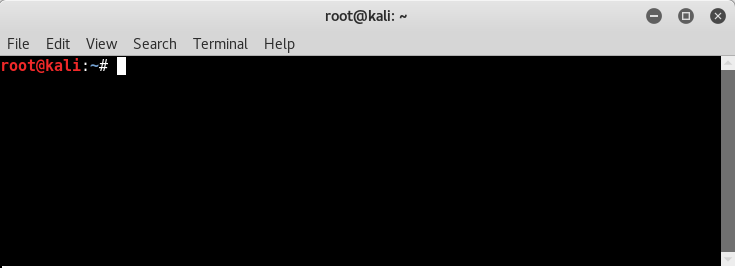
\includegraphics[width=0.9\textwidth]{images/prep/terminalpic.png}
		\caption{Terminal in Kali}
		\label{fig:terminal kali}
	\end{figure}

Zuerst muss hier der folgende Befehl eingegeben werden. (Beachten Sie die Englische Tastatureinstellung)
\begin{lstlisting}
fdisk -l
\end{lstlisting}
Hier sollte eine ähnliche Ausgabe wie hier im Bild folgen. 

	\begin{figure}[H]
		\centering
		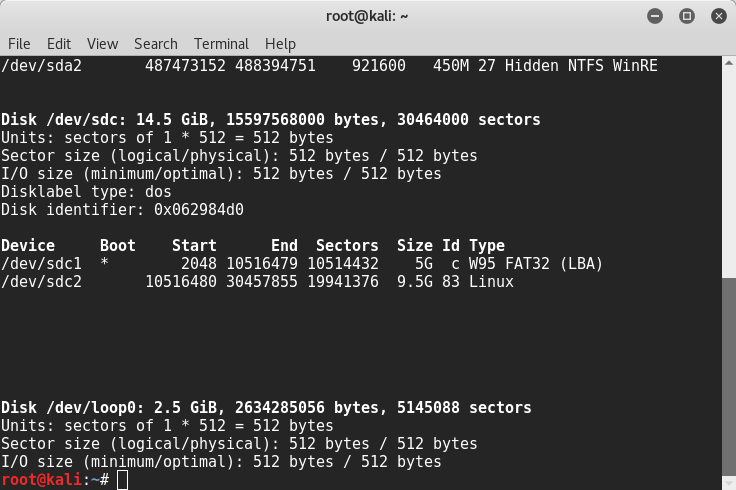
\includegraphics[width=0.9\textwidth]{images/prep/fdisk.png}
		\caption{Ausgabe fdisk -l}
		\label{fig:fdsik output}
	\end{figure}

Nun muss unser USB-Stick unter den Devices gefunden werden. Achten sie dabei darauf, dass der USB-Stick zwei Partitionen besitzt. Zusätzlich sollte geprüft werden, ob die beiden Partitionen mit den vorher eingestellten Größen und Dateisystemen übereinstimmen.
Wählen Sie nun die Linux Partition aus. In unserem Beispiel ist das die im Bild markierte sdc2 Partition.

	\begin{figure}[H]
		\centering
		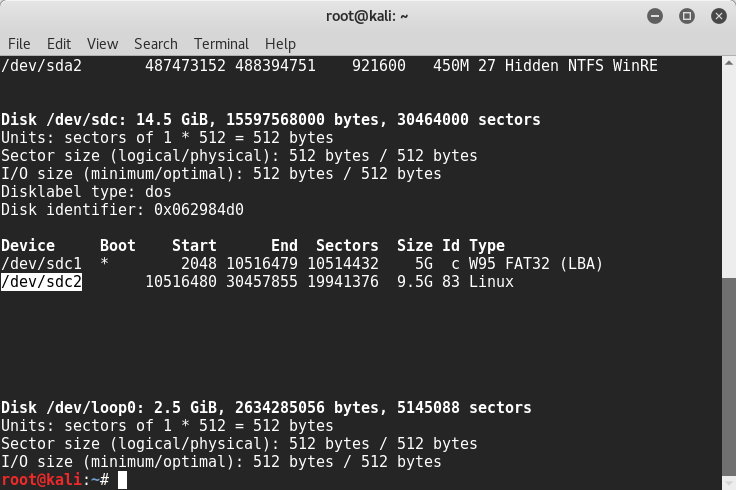
\includegraphics[width=0.9\textwidth]{images/prep/fdisk_marked.png}
		\caption{Finden der richtigen Partition}
		\label{fig:fdisk partition}
	\end{figure}

Um den Stick nun persistent zu machen, geben Sie folgende Befehle ein.
\begin{itemize}
	\item \bashCommand{mkdir -p /mnt/UUI} Erstellen eines Verzeichnisses um den USB-Stick zu mounten.
	\item \bashCommand{mount /dev/sdc2 /mnt/UUI} Ersetzen Sie sdc2 mit ihrer jeweiligen Partition. Dies mountet die Partition auf das erstellte Verzeichnis.
	\item \bashCommand{echo "/ union"> /mnt/UUI/persistence.conf} Dieser Befehl aktiviert die Persistenz indem die Konfigurationdaten hinzugefügt werden.
	\item \bashCommand{umount /dev/sdc2 \&\& reboot}  Ersetzen Sie sdc2 mit ihrer jeweiligen Partition. Die Partition wird unmounted und der PC startet neu.
\end{itemize}

Die von uns geschaffene Security Workbench befindet sich nun in einem öffentlichen Github Repository. Dieses kann mit folgendem Befehl auf den eigenen Rechner geklont werden:
\colorbox{altgray}{\lstinline|git clone https://github.com/th-ingolstadt/INF-M-Projekt-Security-Workbench.git|}
Wurde dieser Befehl ausgeführt sollte eine ähnliche Ausgabe wie hier folgen.

	\begin{figure}[H]
		\centering
		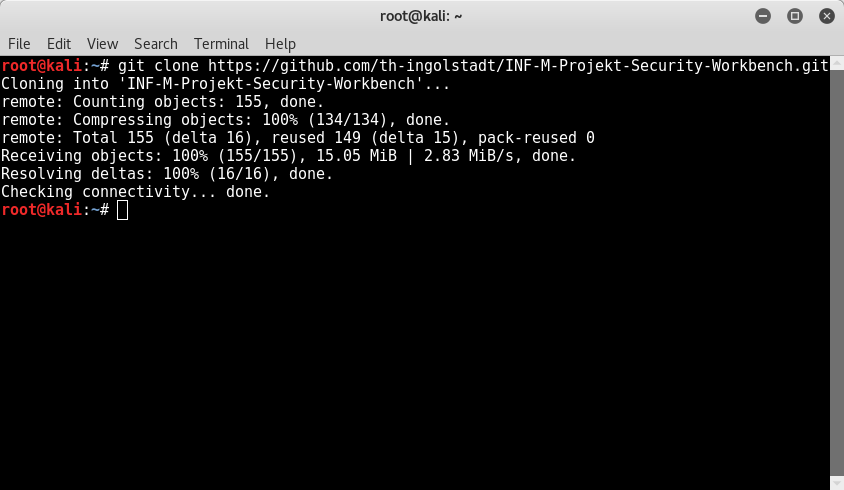
\includegraphics[width=0.9\textwidth]{images/prep/git_clone.png}
		\caption{Ausgabe git clone befehl}
		\label{fig:git clone output}
	\end{figure}
Nachdem der Download abgeschlossen ist, befindet sich der Projektordner im root-Verzeichnis.

\section{Einführung in das Arbeiten mit Linux}
\label{section_startWorkbench}
Um nun mit der Security Workbench arbeiten zu können, muss man diese über das Terminal aufrufen.
Sollte man keine Erfahrung beim Arbeiten mit dem Terminal haben, so kann man hier kurz auf dieser Website die grundlegenden Befehle nachschauen.
\hyperref[Basic Commands]{'http://kali4hackers.blogspot.de/2013/06/some-basic-commands-for-kali-linux.html''}
Um nun die Workbench aufzurufen werden folgende Befehle benötigt:
\begin{itemize}
	\item \bashCommand{cd INF-M-Projekt-Security-Workbench/} mit diesem Befehl wechselt man in das Verzeichnis INF-M-Projekt-Security-Workbench.
	\item \bashCommand{cd Projekte} hiermit wechselt man in das Verzeichnis Projekte. Die beiden cd Befehle können auch zusammengefasst werden. 
	\item \bashCommand{python securityWorkbench.py} Starten des Security-Workbench-Python-Skriptes. Dies startet das Hauptfenster der Workbench.
\end{itemize}

	\begin{figure}[H]
		\centering
		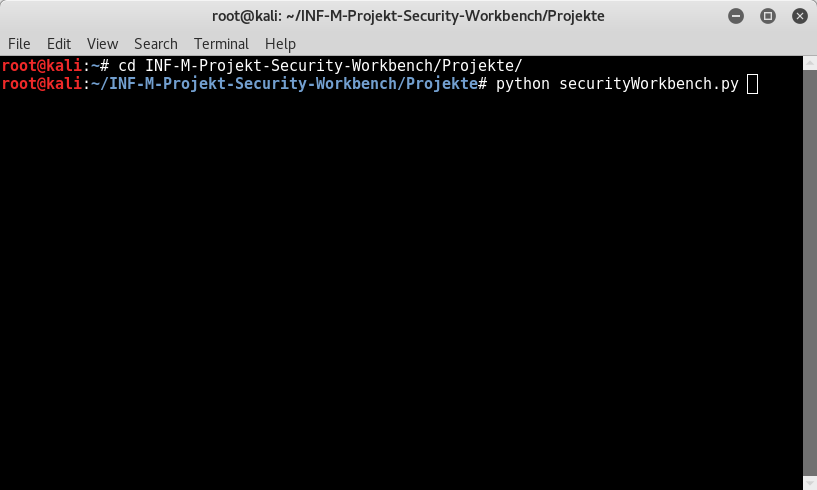
\includegraphics[width=0.9\textwidth]{images/prep/start_the_workbench.png}
		\caption{Start der Workbench mit dem Terminal}
		\label{fig:start workbench with terminal}
	\end{figure}

	\begin{figure}[H]
		\centering
		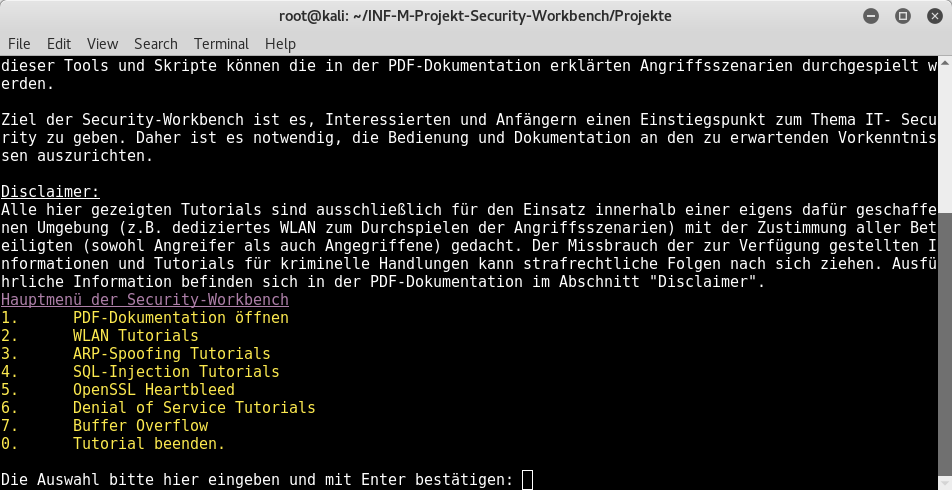
\includegraphics[width=0.9\textwidth]{images/prep/mainwindow_workbench.png}
		\caption{Hauptseite der Workbench}
		\label{fig:maindindow workbench}
	\end{figure}

\section{Weitere Konfigurationen}
Auf den von uns vorbereiteten Kali Live USB-Sticks befindet sich ein Autostartskript.  Dieses öffnet beim Systemstart automatisch die Security Workbench.
\begin{itemize}
	\item \bashCommand{[Desktop Entry]} 
	\item \bashCommand{Name=SecurityWorkBench} 
	\item \bashCommand{Path=/root/INF-M-Projekt-Security-Workbench/Projekte/}
	\item \bashCommand{Exec= python securityWorkbench.py} 
	\item \bashCommand{Terminal=true} 
	\item \bashCommand{Type=Application} 
	\item \bashCommand{X-GNOME-Autostart-enabled=true} 
\end{itemize}
Dieses Skript befindet sich auch in der Workbench im Verzeichnis \colorbox{altgray}{\lstinline|Projekte|}.
Um nun dieses Skript auf Ihrem neu erstellten Kali Live USB-Stick zu aktivieren, geben Sie folgenden Befehl in ein neues Terminal ein.
\colorbox{altgray}{\lstinline|cp -i INF-M-Projekt-Security-Workbench/Projekte/sec.desktop /etc/xdg/autostart/|}.

\begin{itemize}
	\item \bashCommand{cp} Kopieren 
	\item \bashCommand{-i} Interaktives Kopieren, sollte bereits eine Datei mit dem selben Namen am Zielort existieren, wird der Benutzer gefragt, ob er diese überschreiben will. 
	\item \bashCommand{INF-M-Projekt-Security-Workbench/Projekte/sec.desktop} Pfad der zu kopierenden Datei.
	\item \bashCommand{/etc/xdg/autostart/} Pfad des Verzeichnisses, in welches die Datei kopiert wird.
\end{itemize}
Beim nächsten Systemstart wird nun automatisch die Hauptseite der Security Workbench im Terminal angezeigt. 